\section{Uzyskane wyniki i ich analiza}

\subsection{Eksperyment 1}

\par Na początku, postanowiono zbadać wyniki uzyskane poprzez uruchomienie systemu w wersji bazowej. W procesie decyzyjny nie są brane pod uwagę żadne dane kontekstowe, poza dystansem między patrolem, a wybranym incydentem. Konfiguracja została przedstawiona w tabeli \ref{tab:eksperyment1Konfiguracja}.

\begin{table}[H]
    \centering
    \begin{tabular}{|c|c|}
        \hline
        Nazwa parametru & Wartość \\
        \hline
        \hline
         \texttt{EvenPatrolDistribution} & \texttt{True} \\
         \hline
         \texttt{DistanceWeight} & $1$ \\
         \hline
         \texttt{SameDistrictWeight} & $0$ \\
         \hline
         \texttt{InsufficientNumberOfPatrolsInDistrictWeight} & $0$ \\
         \hline
    \end{tabular}
    \caption{Eksperyment 1 - Konfiguracja}
    \label{tab:eksperyment1Konfiguracja}
\end{table}

Wyniki zostały przedstawione w tabeli \ref{tab:eksperyment1Wyniki}. Dodatkowo na grafice \ref{fig:eksperyment1IloscIncydentowWCzasie} widoczny jest przebieg symulacji.

\begin{table}[H]
    \centering
    \begin{tabular}{|c|c|c|p{0.2\linewidth}|p{0.2\linewidth}|}
        \hline
        Uruchomienie & Ilość incydentów & Ilość strzelanin & Średni dystans rozważanego patrolu od incydentu & Średni dystans wybranego patrolu od incydentu \\
        \hline
        \hline
        1 & 143 & 5 & 7185.31m & 3002.58m \\
        \hline
        2 & 120 & 5 & 7227.53m & 3961.69m \\
        \hline
        3 & 131 & 6 & 6377.79m & 3629.75m \\
        \hline
        \hline
        \textbf{Średnie} & \textbf{131.33} & \textbf{5.33} & \textbf{6930.21m} & \textbf{3531.34m} \\
        \hline
    \end{tabular}
    \caption{Eksperyment 1 - Wyniki}
    \label{tab:eksperyment1Wyniki}
\end{table}

\begin{figure}[H]
    \centering
    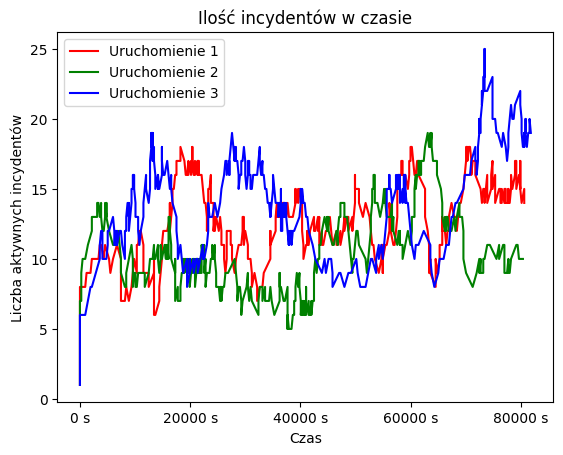
\includegraphics[width=\linewidth]{Experiment 1 - Incidents In Time}
    \caption{Eksperyment 1 - Ilość incydentów w czasie}
    \label{fig:eksperyment1IloscIncydentowWCzasie}
    \source{Opracowanie Własne}
\end{figure}

\subsection{Eksperyment 2}

\par Następnie postanowiono sprawdzić, w jaki sposób na symulację wpłynie sposób przypisania patroli. Zrezygnowano z równomiernego ich rozłożenia, na rzecz priorytetyzacji dzielnic z większym poziomem zagrożenia. Konfiguracja ta jest przedstawiona w tabeli \ref{tab:eksperyment2Konfiguracja}.

\begin{table}[H]
    \centering
    \begin{tabular}{|c|c|}
        \hline
        Nazwa parametru & Wartość \\
        \hline
        \hline
         \texttt{EvenPatrolDistribution} & \texttt{False} \\
         \hline
         \texttt{DistanceWeight} & $1$ \\
         \hline
         \texttt{SameDistrictWeight} & $0$ \\
         \hline
         \texttt{InsufficientNumberOfPatrolsInDistrictWeight} & $0$ \\
         \hline
    \end{tabular}
    \caption{Eksperyment 2 - Konfiguracja}
    \label{tab:eksperyment2Konfiguracja}
\end{table}

Wyniki zostały przedstawione w tabeli \ref{tab:eksperyment2Wyniki}. Dodatkowo na grafice \ref{fig:eksperyment2IloscIncydentowWCzasie} widoczny jest przebieg symulacji.

\begin{table}[H]
    \centering
    \begin{tabular}{|c|c|c|p{0.2\linewidth}|p{0.2\linewidth}|}
        \hline
        Uruchomienie & Ilość incydentów & Ilość strzelanin & Średni dystans rozważanego patrolu od incydentu & Średni dystans wybranego patrolu od incydentu \\
        \hline
        \hline
        1 & 133 & 5 & 5216.66m & 3758.80m \\
        \hline
        2 & 113 & 6 & 6790.06m & 3483.38m \\
        \hline
        3 & 97 & 1 & 6630.84m & 2881.52m \\
        \hline
        \hline
        \textbf{Średnie} & \textbf{114.33} & \textbf{4} & \textbf{6212.52m} & \textbf{3374.57m} \\
        \hline
    \end{tabular}
    \caption{Eksperyment 2 - Wyniki}
    \label{tab:eksperyment2Wyniki}
\end{table}

\begin{figure}[H]
    \centering
    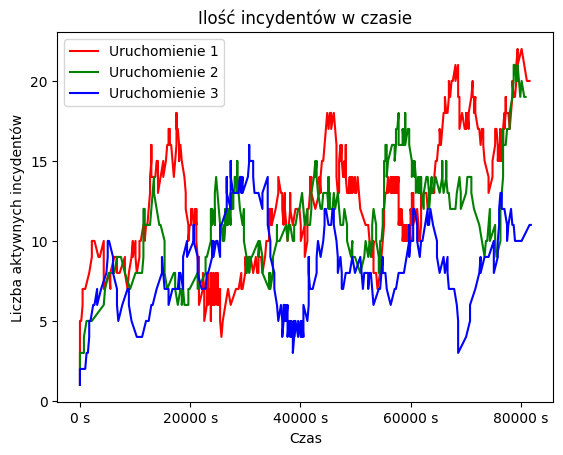
\includegraphics[width=\linewidth]{Experiment 2 - Incidents In Time}
    \caption{Eksperyment 2 - Ilość incydentów w czasie}
    \label{fig:eksperyment2IloscIncydentowWCzasie}
    \source{Opracowanie Własne}
\end{figure}

\subsection{Eksperyment 3}

\par Na samym końcu postanowiono włączyć do mechanizmu decyzyjnego informacje o relacji patrolu z daną dzielnicą, jak i o obecnym stanie dzielnicy, do której dany patrol jest przypisany. Konfiguracja ta została przedstawiona w tabeli \ref{tab:eksperyment3Konfiguracja}.

\begin{table}[H]
    \centering
    \begin{tabular}{|c|c|}
        \hline
        Nazwa parametru & Wartość \\
        \hline
        \hline
         \texttt{EvenPatrolDistribution} & \texttt{False} \\
         \hline
         \texttt{DistanceWeight} & $1$ \\
         \hline
         \texttt{SameDistrictWeight} & $1$ \\
         \hline
         \texttt{InsufficientNumberOfPatrolsInDistrictWeight} & $1$ \\
         \hline
    \end{tabular}
    \caption{Eksperyment 3 - Konfiguracja}
    \label{tab:eksperyment3Konfiguracja}
\end{table}

Wyniki zostały przedstawione w tabeli \ref{tab:eksperyment3Wyniki}. Dodatkowo na grafice \ref{fig:eksperyment3IloscIncydentowWCzasie} widoczny jest przebieg symulacji.

\begin{table}[H]
    \centering
    \begin{tabular}{|c|c|c|p{0.2\linewidth}|p{0.2\linewidth}|}
        \hline
        Uruchomienie & Ilość incydentów & Ilość strzelanin & Średni dystans rozważanego patrolu od incydentu & Średni dystans wybranego patrolu od incydentu \\
        \hline
        \hline
        1 & 86 & 3 & 7308.25m & 3175.75m \\
        \hline
        2 & 124 & 4 & 7110.08m & 3602.15m \\
        \hline
        3 & 115 & 1 & 6236.87m & 2868.57m \\
        \hline
        \hline
        \textbf{Średnie} & \textbf{108.33} & \textbf{2.67} & \textbf{6885.07m} & \textbf{3215.49m} \\
        \hline
    \end{tabular}
    \caption{Eksperyment 3 - Wyniki}
    \label{tab:eksperyment3Wyniki}
\end{table}

\begin{figure}[H]
    \centering
    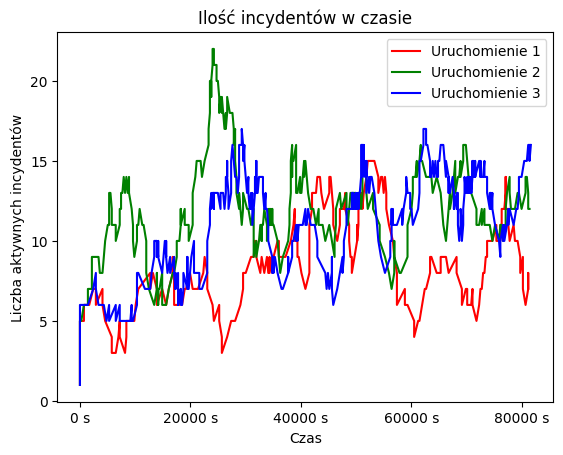
\includegraphics[width=\linewidth]{Experiment 3 - Incidents In Time}
    \caption{Eksperyment 3 - Ilość incydentów w czasie}
    \label{fig:eksperyment3IloscIncydentowWCzasie}
    \source{Opracowanie Własne}
\end{figure}

\subsection{Analiza}

\par Uzyskane wyniki pokazują, że wykorzystywanie danych kontekstowych w procesie decyzyjnym może mieć pozytywny wpływ na rezultaty działania systemu. Jest to dobrze widoczne, na podstawie tabeli \ref{tab:zestawienieWynikowEksperymentow}, gdzie coraz lepsze rezultaty średniego dystansu dla wybranego patrolu zostały uzyskane wraz z włączaniem kolejnych danych kontekstowych do działania systemu.

\par Pozytywna zmiana w średnim dystansie patrolu od incydentu widoczna pomiędzy eksperymentem 1 i 2 wynika z faktu, iż więcej patroli jest powiązanych z dzielnicami, w których pojawiają się incydenty. Zaowocowało to również pozytywną zmianą w kontekście tego, jaką drogę musi pokonać wybrany patrol.

\par W wynikach eksperymentu numer 3, widzimy ponowny wzrost w średnim dystansie patrolu od incydentu, jednak wciąż mniejszy, niż w przypadku eksperymentu 1 i równomiernego rozłożenia patroli. Oznacza to, że patrole nie były tak skupione w poszczególnych dzielnicach, a bardziej równomiernie rozłożone na całym dostępnym obszarze. Wynika to z tego, iż patrole znajdujące się w bezpiecznych i normalnych dzielnicach, mogły zostać wybierane do rozwiązywania incydentów w niepowiązanych dzielnicach, jednak znajdujących się niedaleko, na przykład sąsiadujących. Pozwoliło to na zmniejszenie średniego dystansu wybranego patrolu od incydentu. Rezultaty tego możemy zaobserwować porównując wykresy przebiegów symulacji, gdzie widzimy, że eksperyment numer 3 poradził sobie najlepiej, zachowując ilość aktywnych w danym momencie incydentów pod kontrolą - ilość ta była poniżej granicy dwudziestu, czyli ilości patroli, jaka działała w systemie.

\begin{table}[H]
    \centering
    \begin{tabular}{|p{0.16\linewidth}|p{0.16\linewidth}|p{0.16\linewidth}|p{0.16\linewidth}|p{0.16\linewidth}|}
        \hline
        Eksperyment & Średnia ilość incydentów & Średnia ilość strzelanin & Średni dystans rozważanego patrolu od incydentu & Średni dystans wybranego patrolu od incydentu \\
        \hline
        \hline
        Eksperyment 1 & 131.33 & 5.33 & 6930.21m & 3531.34m \\
        \hline
        Eksperyment 2 & 114.33 & 4 & 6212.52m & 3374.57m \\
        \hline
        Eksperyment 3 & 108.33 & 2.67 & 6885.07m & 3215.49m \\
        \hline
    \end{tabular}
    \caption{Zestawienie wyników eksperymentów}
    \label{tab:zestawienieWynikowEksperymentow}
\end{table}